\documentclass[]{article}

\usepackage{pgf-pie}
\usepackage{url}
\usepackage[utf8]{inputenc}

\title{Natural Language processing for Knowledge Representation} \author{Jens
  Claes}

\newcommand{\example}[1]{\textit{``#1''}}

\begin{document}

\maketitle

\section{Probleemstelling}
\paragraph{} Bedrijfsprocessen worden geregeld door specificaties. Deze worden vaak geschreven in een natuurlijke taal, door een domein expert. Vervolgens worden deze specificaties vertaald naar uitvoerbare programma's. Bij deze vertaling slopen er vaak fouten in. Bovendien zijn er vaak meerdere programma's die elk opnieuw de specificatie moeten implementeren. Zo ontstaan er niet allen inconsistenties met de specificatie, maar ook tussen de verschillende programma's onderling zijn er inconsistenties. Ten slotte is het moeilijke om de specificatie achteraf nog aan te passen omdat alle programma's dan aangepast moeten worden.

\paragraph{} Het antwoord van de academische wereld op deze problemen, zijn \textit{Knowledge Base Systems} (KBS). In dit paradigma worden de specificaties in natuurlijke taal vertaald naar specificaties in een formele taal. Deze formele specificatie wordt gebruikt in alle programma's. Zo is het niet meer mogelijk dat de programma's onderling inconsistent zijn. Ze gebruiken namelijk allemaal de formele specificatie. Daardoor is ook het aanpassen van de specificatie makkelijker. Enkel de formele specificatie moet aangepast worden, de programma's blijven hetzelfde.

\paragraph{} Het probleem met deze aanpak is dat er nog steeds een vertaling moet gebeuren van natuurlijke taal naar een formele taal. De specificatie in natuurlijke taal wordt vaak opgesteld door een domein expert die formele talen niet machtig is. De formele specificatie wordt dan weer opgesteld door een KBS expert. Deze persoon kent formele talen maar heeft een beperkte kennis van het domein. Door deze mismatch van kennis, is de feedback loop tussen de twee experten beperkt. Het is dus nog steeds mogelijk dat er fouten sluipen in de vertaling.

\paragraph{} De vraag rijst dus of we een formele taal kunnen ontwerpen die toegankelijk is voor domein experten, rijk genoeg is voor praktische problemen en toepasbaar is binnen het KBS paradigma.

\paragraph{} Deze thesis onderzoekt of een formele natuurlijke taal het antwoord is op die vraag. Natuurlijke taal wordt immers al gebruikt bij het opstellen van de specificatie. Figuur \ref{fig:natural-language-use} toont het gebruik van natuurlijke taal in vereistenanalyse in 1999. Slechts 5 procent werd toen in een formele taal opgesteld. 16 procent werd in gestructureerde natuurlijke taal opgesteld. Dit wil zeggen dat de specificatie in een natuurlijke taal is opgesteld maar slechts een beperkt aantal zinsconstructies zijn toegestaan, om de leesbaarheid te verhogen.

\begin{figure}
  \label{fig:natural-language-use}
  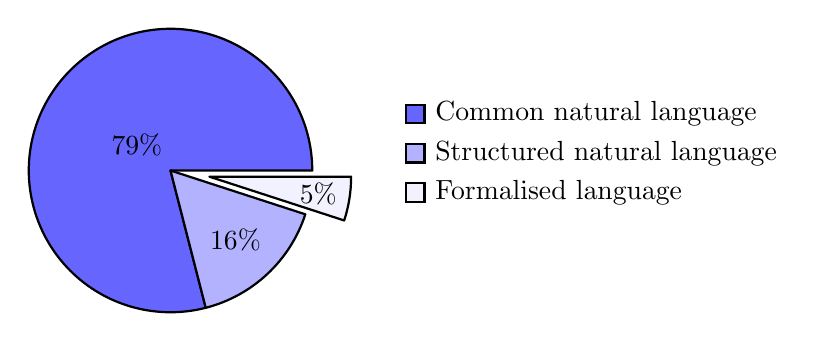
\begin{tikzpicture}
      \pie[text = legend, radius = 1.8, explode = {0, 0, 0.5}, color = {blue!60, blue!30, blue!5}]{79/Common natural language, 16/Structured natural language, 5/Formalised language}
  \end{tikzpicture}
  \caption{Gebruik van natuurlijke taal in vereistenanalyse in 1999 (van figuur 5 in \cite{Luisa2004})}
\end{figure}

\paragraph{} In deze thesis ontwerpen we een nieuwe gestructureerde natuurlijke taal (vanaf nu CNL genoemd naar de Engelse term Controlled Natural Language). Het doel van deze taal is dat ze leesbaar is voor de domein expert, de KBS expert en computers. Zo kan een programma de formele specificatie opstellen vanuit de specificatie in de natuurlijke taal. Er is dan nog maar 1 bron van waaruit alles geregeld wordt. Inconsistenties zijn niet meer mogelijk. Bovendien kan men nog steeds makkelijk de specificatie aanpassen.

\section{Literatuurstudie}
In het verleden zijn er al meerdere pogingen gedaan om teksten in natuurlijke taal te transformeren naar formele modellen.

\paragraph{Circe} Zo wordt de tool Circe\cite{Ambriola1997} gebruikt in vereistenanalyse. De gebruiker moet een vocabularium, een set van substitutie regels en een specificatie in natuurlijke aanleveren. De tool probeert dan steeds de beste regel te vinden om zo de tekst geleidelijk aan te transformeren naar een formeel model. Het grote voordeel van de methode is dat er regelsets bestaan voor meerdere soorten modellen: data flow modellen, entity-relationship modellen, ...

Verder is het in Circe mogelijk om in het vocabularium woorden te taggen. De regels kunnen hier dan gebruik van maken om te bepalen of ze van toepassing zijn op bepaalde zinnen. Op die manier introduceert Circe types in het vocabularium.

Een voorbeeld (uit \cite{Ambriola1997}): \example{bron/UIT STUURT data/INFO NAAR doel/IN}. De woorden \example{stuurt} en \example{naar} liggen vast in de regelset. De andere 3 woorden komen uit het vocabularium. Deze moeten een bepaalde tag hebben om te matchen met de regel. 

\paragraph{ACE} Attempto Controlled English (ACE)\cite{Fuchs2008} is een gestructureerde taal voor kennisrepresentatie. Het is een subset van Engels die naar een subset van eerste-orde-logica vertaald. Het is echter wel een formele taal: elke zin in ACE heeft slechts één betekenis, ook al is de Engelse zin ambigu. Om de juiste betekenis te kennen, kan men gebruik maken van de parafraseertool van ACE. Deze tool zet de interne representatie terug om naar één of meerdere zinnen in ACE. Op die manier kan men niet alleen de betekenis van de zin leren, maar ook de taal zelf.

ACE is een general purpose CNL: Het bevat een ingebouwd vocabularium. De gebruiker moet dus zelf geen vocabularium opstellen en kan direct beginnen met het schrijven van de specificatie. Het nadeel aan deze aanpak is dat ACE dus ook geen domeinkennis kan gebruiken voor het analyseren van de zinnen. Sommige constructies moeten daarom met een koppelteken geschreven worden. Zo wordt er in \cite{ACEConstructionRules} het voorbeeld gegeven van \example{A student is interested-in a course} en \example{A student is interested in a classroom}.

Op die manier probeert ACE sommige ambiguïteiten op te lossen. Een gelijkaardige truk wordt bijvoorbeeld ook gebruikt om de voorrang van \example{en} en \example{of} op te lossen. Standaard heeft \example{en} voorrang. Maar als de \example{en} voorafgegaan wordt door een komma, dan heeft \example{of} voorrang. \cite{ACEConstructionRules} geeft het voorbeeld \example{A client \{enters a red card or enters a blue card\}, and enters a code.}

In andere gevallen kiest ACE gewoon hoe de zin geïnterpreteerd moet worden op basis van een set van \textit{interpration rules}. Zo slaat de \example{manually} in \example{A customer who {enters a card manually} types a code.}\cite{ACEConstructionRules} op \example{enters} en niet op \example{types} omdat een bijwoord bij voorkeur achter het werkwoord staat.

Één van de sterke punten van ACE is het oplossen van anaforische referenties (referenties naar woorden eerder in de zin of naar woorden van vorige zinnen). De invoertekst wordt namelijk als één geheel vertaald. Daardoor is het niet nodig om lange zinnen te schrijven met veel bijzinnen. Men kan zo'n zinnen namelijk opbreken in een aantal kortere zinnen. Zo kan \example{A customer inserts a card that carries a code.} geschreven worden als \example{A card carries a code. A customer inserts the card.}\cite{Fuchs2008}. Op deze manier kan de specificatie veel leesbaarder gehouden worden.

Origineel was ACE bedoeld voor het opstellen van specificaties voor software. Ondertussen kent de taal al meerdere toepassingen, in verschillende domeinen. Er zijn ook meerdere tools die overweg kunnen met ACE als input.

Zo is er de Attempto Parsing Engine APE die ACE zinnen omzet naar Discourse Representation Structures (DRS). Deze variant op eerste-orde-logica wordt vooral gebruikt om makkelijker te acherhalen naar wat de anaforische referenties refereren. APE geeft ook een parafrasering van de invoertekst. Zodat de gebruiker kan controleren of de tool de tekst op de juiste manier leest. Bovendien kan APE waarschuwingen geven bij mogelijke problemen. Bijvoorbeeld het gebruik van een bepaald lidwoord zonder een antecedent waarnaar de noun phrase kan verwijzen.

Verder is er ook de Attempto Reasoner RACE. Deze tool kan controleren of een specificatie consistent is met zichzelf. De tool zal dan zeggen welke zinnen met elkaar in conflict zijn. Op die manier weet de gebruiker dat er een fout is en waar deze zich ongeveer bevindt. De tool kan ook vragen in natuurlijke taal beantwoorden. RACE antwoordt niet alleen op de vraag maar geeft ook de zinnen die nodig zijn om te bewijzen dat het gegeven antwoord juist is. Ten slotte kan RACE bewijzen of een bepaalde zin het logische gevolg is van de specificatie. Op die manier kan de gebruiker testen of de specificatie correct is.

APE en RACE zijn de twee belangrijkste tools. Er zijn er echter nog veel meer. Zo is er de ACE View Protégé plug-in. Dit is een plugin die de vertaling tussen OWL en ACE doet binnen de Protégé-omgeving (een editor voor het maken van ontologiën). Op die manier ziet de gebruiker enkel ACE zinnen en hoeft dus de formele OWL taal niet te kennen om met bestaande modellen om te gaan of om nieuwe modellen te maken. Ten slotte is er ook nog AceRules. Hiermee kan de gebruiker de zinnen die geïmpliceerd worden door de specificatie te weten komen.

Over het algemeen is ACE een zeer uitgebreide taal. Veel Engelse zinnen zijn ook geldige ACE zinnen, echter niet allemaal. Dit zorgt ervoor dat het soms niet duidelijk is welke zinnen geldig zijn en welke niet. Volgens \cite{Fuchs2008} heeft een gebruiker 2 dagen nodig om de taal te leren.

\paragraph{PENG} Andere talen zoals PENG\cite{Schwitter2002} zijn makkelijker om te leren. PENG is ook een CNL die vertaald naar DRS structuren. In tegenstelling tot ACE bevat PENG geen groot ingebouwd lexicon. De gebruiker moet zelf de woorden aanbrengen die gebruikt worden. De gebruiker kan dit doen tijdens het bewerken en moet dus niet op voorhand aangeven wat het lexicon is. De categorieën voor deze domeinspecifieke woorden zijn: zelfstandig naamwoord, bijvoeglijk naamwoord, werkwoord en bijwoord. PENG biedt ook de mogelijkheid om synoniemen of afkortingen te introduceren. Op die manier kan de tekst leesbaarder gemaakt worden. Naast de domeinspecifieke woorden kent PENG ook een aantal functionele woorden die ingebakken zitten in de taal. Deze woorden helpen PENG om de zinsconstructies te herkennen.

Net zoals ACE kent PENG het principe van constructieregels en interpretatieregels. De constructieregels bepalen welke zinnen deel zijn van de taal. Bij PENG zijn deze regels eenvoudiger omdat de taal zeer simpel gehouden is. Op die manier willen ze het makkelijker maken om zinnen te maken in de taal. Over het algemeen lijken de constructieregels van PENG en ACE veel op elkaar.

De interpretatieregels bepalen hoe de zin vertaald wordt naar logica. Zo is er een interpretatieregel voor hoe anaforische referenties opgelost worden. Deze regel is gelijkaardig in ACE en PENG. Andere regels bepalen welke functiewoorden sterker binden. Zowel ACE als PENG gebruiken hiervoor dezelfde volgorde als in eerste-orde-logica. ACE staat wel uitzonderingen toe door het toevoegen van komma's. PENG houdt de taal simpel en staat dit niet toe.

PENG is makkelijker om te leren dan ACE omwille van ECOLE\cite{Schwitter2003}. Deze tool kan suggesties geven over de woordcategorieën die kunnen volgen op een bepaalde zin. Zo geeft \cite{Schwitter2003} het voorbeeld van \example{Een} dat gevolgd kan worden door een \texttt{adjectief} of een \texttt{substantief}. Indien de gebruiker de woordcategorie niet kent, kan hij doorklikken op die categorie voor een aantal mogelijkheden. Op die manier moet de gebruiker enkel de woordcategorieën leren en niet de geldige zinsconstructies.

Naast de suggestietool bevat PENG, net zoals ACE, ook een parafraseertool. Deze tool herschrijft de invoer zodat het duidelijker is hoe PENG de zin begrepen heeft. Anaforische referenties worden bijvoorbeeld omgezet in de noun phrase naarwaar ze verwijzen.

Net zoals in ACE is het ook in PENG mogelijk om te controleren of een specificatie consistent is\cite{Schwitter2004b}. Daarnaast is het ook mogelijk om te controleren op redundantie. Indien een zin al door een andere zin geïmpliceerd wordt, hoeft deze niet expliciet deel uit te maken van de specificatie. Op die manier kan de specificatie kort gehouden worden, wat de leesbaarheid verhoogd.

Naast de general purpose CNL bevat PENG ook een subset specifiek voor het semantische web: PENG-D\cite{Schwitter2004}. Deze subset is wel beslisbaar en kan vertaald worden naar description logic, een subset van eerste-orde-logica. PENG-D kan dus gezien worden als het alternatief voor de ACE View Protégé plug-in.
\cite{Schwitter2006} vermeldt drie klassieke manieren van voorstellen van een ontologie (N-Triples, RDF/XML en OWL Abstract) en toont dan verder aan dat PENG een vierde manier is om hetzelfde voor te stellen. De paper toont dit aan door verschillende constructies uit OWL te mappen op zinnen in PENG. Het grote voordeel van PENG t.o.v. de andere voorstellingswijzen is dat PENG ook leesbaar en begrijpbaar is voor de mens.

\paragraph{Implementatie}

% TODO: Feature structures in prolog == ???: http://cs.union.edu/~striegnk/courses/nlp-with-prolog/html/index.html
% TODO: Korte samenvatting van ACE en PENG en dan vooral vergelijken
% TODO: Ander werk even kort voorstellen.
% TODO: ~15 papers is genoeg als referenties

\subsection{Todo}
\begin{enumerate}
  \item ACE\cite{Fuchs2008} Niet: \cite{Fuchs}, Master Thesis\cite{Dellis2010} 
  \item PENG\cite{Schwitter2002, Schwitter2004b, Schwitter2003, Schwitter2006}, PENG Light\cite{Schwitter2008, White2009},
    PENG D\cite{Schwitter2004}, ook van Schwitter:\cite{Schwitter2005} 
  \item Writing support for CNL's\cite{Kuhn2008} 
  \item Model checking\cite{Flake2002, Konrad2005, Nelken, Jak2008}
  \item Lijst van ambiguïteiten \cite{Berry2003} 
  \item RuleSpeak\cite{Ross2009a, Ross2013, Ross2013a, Ross2009} 
  \item RuleCNL\cite{Njonko2014} 
  \item CELT\cite{Pease2010, Dellis2010}
  \item Overzicht + classificatie\cite{Kuhn2014}
  \item Evaluation CNL\cite{Kuhn2010}
  \item A principled approach to CNL's\cite{Kuhn2013} 
  \item SBVR\cite{Spreeuwenberg2010, Levy2013} 
\end{enumerate}
			

\section{Planning}
TODO: Write

\section{Referenties}
\bibliographystyle{unsrt}
\bibliography{tekst}

\end{document}


% LocalWords: KBS Systems Knowledge programma's
